% ══════════════════════════════════════════════════════════════
% SCORED 2026 — Workshop Paper (6 pages, ACM sigconf format)
% Software Supply Chain Offensive Research and Ecosystem Defenses
% Co-located with ACM CCS 2026, The Hague, Netherlands
% Single-anonymous review (authors are visible)
% ══════════════════════════════════════════════════════════════
\documentclass[sigconf,nonacm]{acmart}
% Note: use [sigconf] without nonacm for camera-ready if accepted

\usepackage{booktabs}
\usepackage{listings}
\usepackage{tikz}
\usetikzlibrary{arrows.meta, positioning, shapes.geometric}
\usepackage{pgfplots}
\pgfplotsset{compat=1.18}

% Remove ACM-specific metadata for submission draft
\settopmatter{printacmref=false}
\renewcommand\footnotetextcopyrightpermission[1]{}
\pagestyle{plain}

\begin{document}

\title{From Fix Commits to Vulnerable Functions: Automated Patch Mining for Function-Level CVE Resolution}

\author{Anonymous Author 1}
\affiliation{
    \institution{Anonymous Institution}
    \city{Anonymous City}
    \country{Anonymous Country}
}
\email{anon1@anonymous.edu}

\author{Anonymous Author 2}
\affiliation{
    \institution{Anonymous Institution}
    \city{Anonymous City}
    \country{Anonymous Country}
}
\email{anon2@anonymous.edu}

% ──────────────────────────────────────────────────────────────
\begin{abstract}
Vulnerability databases report security advisories at the package-version
level, but reachability-based security tools require \emph{function-level}
data to determine whether a vulnerability is actually exercised by downstream
consumers.
We present an automated, multi-language patch mining technique that extracts
affected function names from fix commits linked to GitHub Security Advisories
(GHSA) and Project~KB.
For each advisory, our pipeline fetches the fix commit diff via the GitHub
API, applies language-aware regex patterns for JavaScript, Python, and Java,
and maps extracted names to static call graphs for reachability verification.
We evaluate the technique at two scales: (1)~a precision-focused study of
45~npm and PyPI advisories (69\% yield, 84\% precision, 100\% reachability
confirmation); and (2)~a large-scale recall study against the SAP Project~KB
gold standard, processing all 1{,}248 Java vulnerability statements and
achieving an 86.0\% extraction rate on fetchable fix-commit diffs, recovering
8{,}069 unique function names.
We characterize failure modes across both ecosystems and discuss implications
for improving vulnerability database reporting in software supply chains.
\end{abstract}

\begin{CCSXML}
<ccs2012>
<concept>
<concept_id>10011007.10011074.10011099.10011102.10011103</concept_id>
<concept_desc>Software and its engineering~Software maintenance tools</concept_desc>
<concept_significance>500</concept_significance>
</concept>
<concept>
<concept_id>10002978.10003029.10011703</concept_id>
<concept_desc>Security and privacy~Software security engineering</concept_desc>
<concept_significance>500</concept_significance>
</concept>
</ccs2012>
\end{CCSXML}

\ccsdesc[500]{Software and its engineering~Software maintenance tools}
\ccsdesc[500]{Security and privacy~Software security engineering}

\keywords{software supply chain, vulnerability, patch mining, call graph, 
CVE, function-level analysis}

\maketitle

% ══════════════════════════════════════════════════════════════
\section{Introduction}
\label{sec:intro}

Software supply-chain attacks have surged in both frequency and 
impact~\cite{ohm2020backstabber,ladisa2023taxonomy}, prompting widespread 
adoption of Software Composition Analysis (SCA) tools that alert developers 
when a dependency version appears in a vulnerability database. However, 
these tools report at the \emph{package-version} level: they tell an 
engineer that \texttt{qs@6.14.0} has CVE-2022-24999, but not 
\emph{which function} contains the vulnerability.

This granularity gap creates two practical problems:

\begin{enumerate}
    \item \textbf{False-positive overload.} Many flagged CVEs reside in 
    functions that are never called by the downstream 
    application~\cite{pashchenko2020qualitative}. Without function-level 
    data, SCA tools cannot perform reachability filtering, leading to alert 
    fatigue.
    \item \textbf{Missing triage context.} Security engineers reviewing 
    dozens of CVE alerts cannot prioritize effectively without knowing 
    whether the vulnerable function is a core parser (high risk) or an 
    unused utility (low risk).
\end{enumerate}

Manually curated datasets like Project~KB~\cite{ponta2019projectkb} provide
function-level mappings for approximately 1{,}248 Java vulnerability
statements, but manual curation does not scale to the tens of thousands of
advisories across multiple ecosystems.
No automated, multi-language technique exists for extracting function-level
vulnerability data from the information already available in vulnerability
databases.

We observe that fix commits linked to security advisories contain precisely
the information needed: the diff of a security fix structurally reveals
which functions were modified to address the vulnerability.
We present an automated \emph{patch mining} technique that exploits this
observation across three ecosystems (JavaScript, Python, Java), evaluating
both precision against manually validated samples and recall against the
Project~KB gold standard.

\textbf{Contributions.} This paper makes the following contributions:
\begin{itemize}
    \item A multi-language patch mining pipeline supporting JavaScript,
    Python, and Java, requiring no AST parser and operating directly on
    unified diff output.
    \item A precision study on 45~npm and PyPI advisories demonstrating
    69\% yield, 84\% precision, and 100\% reachability confirmation for
    mined functions.
    \item A large-scale recall study against Project~KB: processing all
    1{,}248 Java vulnerability statements achieves 86.0\% extraction
    rate on fetchable diffs, recovering 8{,}069 unique function names.
    \item A failure taxonomy characterizing addressable and inherent
    failure modes across three language ecosystems.
    \item An open replication package with all extracted data, scripts,
    and Project~KB cross-validation results.
\end{itemize}

% ══════════════════════════════════════════════════════════════
\section{Background and Motivation}
\label{sec:background}

\subsection{The Function-Level Data Gap}

Vulnerability databases such as the National Vulnerability Database
(NVD)~\cite{nvd}, the Open Source Vulnerabilities database
(OSV)~\cite{osv}, and GitHub Security Advisories (GHSA) report
vulnerabilities at the package-version level.
For example, GHSA-2022-24999 reports that \texttt{qs} versions prior to
6.9.7 are vulnerable to prototype pollution, but specifies no function name.
A developer whose application calls \texttt{qs.parse()} cannot determine
whether the vulnerable code path is exercised without either manual
inspection of the fix diff or a pre-existing function-level mapping.

Project~KB~\cite{ponta2019projectkb} is the closest prior work: a manually
curated dataset of 1{,}248 Java vulnerability statements, each linked to a
fix commit and optionally to the specific affected construct.
Project~KB demonstrates that function-level data is both feasible and
valuable, but requires expert manual effort that does not scale beyond
a single language.
Table~\ref{tab:db-comparison} compares the granularity offered by major
vulnerability databases.

\begin{table}[t]
    \centering
    \caption{Granularity of vulnerability data across major databases.}
    \label{tab:db-comparison}
    \begin{tabular}{lccc}
        \toprule
        \textbf{Source} & \textbf{Fix commit} & \textbf{Function-level} & \textbf{Scale} \\
        \midrule
        NVD        & rarely   & never    & 200k+ CVEs \\
        OSV        & sometimes & rarely  & 50k+ advisories \\
        GHSA       & often    & never    & 10k+ advisories \\
        Project~KB & always   & manually & 1{,}248 (Java) \\
        \textbf{Ours} & \textbf{always} & \textbf{auto} & \textbf{multi-lang} \\
        \bottomrule
    \end{tabular}
\end{table}

\subsection{Fix Commits as a Data Source}

GHSA advisories increasingly link to the specific fix commit on GitHub.
These fix commits contain a unified diff that reveals exactly which source
files and functions were modified to remediate the vulnerability.
The intuition behind our approach is that a security fix is a structural
proof of the vulnerable function: the developer who wrote the patch knew
exactly which function to change.

% ══════════════════════════════════════════════════════════════
\section{Technique}
\label{sec:technique}

\subsection{Pipeline Overview}

Figure~\ref{fig:pipeline} illustrates the end-to-end patch mining pipeline.

\begin{figure}[t]
\centering
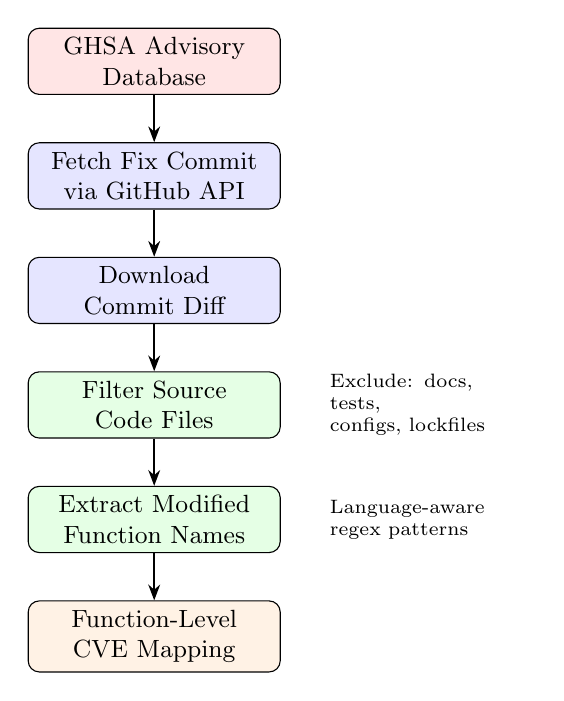
\begin{tikzpicture}[
    node distance=0.6cm,
    box/.style={draw, rounded corners, minimum width=3.2cm, 
                minimum height=0.7cm, align=center, font=\small},
    arrow/.style={-{Stealth[length=2mm]}, thick},
]
\node[box, fill=red!10] (ghsa) {GHSA Advisory\\Database};
\node[box, fill=blue!10, below=of ghsa] (fetch) {Fetch Fix Commit\\via GitHub API};
\node[box, fill=blue!10, below=of fetch] (diff) {Download\\Commit Diff};
\node[box, fill=green!10, below=of diff] (filter) {Filter Source\\Code Files};
\node[box, fill=green!10, below=of filter] (extract) {Extract Modified\\Function Names};
\node[box, fill=orange!10, below=of extract] (output) {Function-Level\\CVE Mapping};

\draw[arrow] (ghsa) -- (fetch);
\draw[arrow] (fetch) -- (diff);
\draw[arrow] (diff) -- (filter);
\draw[arrow] (filter) -- (extract);
\draw[arrow] (extract) -- (output);

% Side annotations
\node[right=0.5cm of filter, font=\scriptsize, text width=2.5cm, align=left] 
    {Exclude: docs, tests,\\configs, lockfiles};
\node[right=0.5cm of extract, font=\scriptsize, text width=2.5cm, align=left] 
    {Language-aware\\regex patterns};
\end{tikzpicture}
\caption{Patch mining pipeline. For each GHSA advisory with a linked fix 
commit, the pipeline downloads the diff, filters to source code changes, and 
extracts modified function definitions.}
\label{fig:pipeline}
\end{figure}

\subsection{Language-Aware Function Extraction}

For each diff hunk in a source code file, we apply language-specific regex
patterns to identify function declarations in modified lines (lines prefixed
with \texttt{+} or \texttt{-} in the unified diff format).
Figure~\ref{fig:regex-patterns} shows representative patterns for all
three supported languages.

\begin{figure}[t]
\begin{lstlisting}[basicstyle=\scriptsize\ttfamily,
                   breaklines=true,
                   frame=single,
                   caption={Language-specific function extraction patterns.
                   Capture group \texttt{(name)} yields the function
                   identifier.},
                   label={fig:regex-patterns}]
# --- JavaScript ---
function\s+(\w+)\s*\(            # named declaration
(\w+)\s*\([^)]*\)\s*\{          # method shorthand
const\s+(\w+)\s*=.*=>           # arrow function
exports\.(\w+)\s*=\s*function   # module export

# --- Python ---
^[+-]\s*(?:async\s+)?def\s+(\w+)\s*\(

# --- Java ---
(?:public|private|protected|\s)\s+
  (?:static\s+)?(?:final\s+)?
  (?:<[^>]+>\s+)?               # generics
  (?:\w+(?:<[^>]+>)?(?:\[\])?)\s+  # return type
  (\w+)\s*\(                    # method name
# Constructors: capital-first identifier
\+?\s+([A-Z]\w+)\s*\([^)]*\)\s*\{
\end{lstlisting}
\end{figure}

All patterns scan lines prefixed with \texttt{+} or \texttt{-} without
requiring a full language parser, making the pipeline robust to incomplete
or syntactically ambiguous diffs common in real-world fix commits.
Java-specific exclusions (test files under \texttt{src/test/}, annotation
lines beginning with \texttt{@}, interface declarations) prevent
non-implementation lines from contributing false extractions.

\subsection{Confidence Scoring}

Each extracted function receives a confidence label:

\begin{itemize}
    \item \textbf{High:} Single function modified in a single source file.
    \item \textbf{Medium:} Multiple functions modified, but one matches 
    security-related naming patterns (\texttt{parse}, \texttt{sanitize}, 
    \texttt{validate}, \texttt{auth}).
    \item \textbf{Low:} Many functions modified across multiple files.
\end{itemize}

\subsection{Reachability Verification}

After extraction, function names are matched against static call graphs
produced by the OSCAR Method Observatory~\cite{oscar-icsme} to determine
whether the mined functions are reachable from the package's public API.
This provides an independent validation signal: if a mined function is
unreachable, it may indicate dead code or a false extraction.

\subsection{End-to-End Walkthrough: CVE-2022-24999}
\label{subsec:walkthrough}

We illustrate the pipeline with a concrete example.
\textbf{CVE-2022-24999} is a prototype pollution vulnerability in \texttt{qs},
a query-string parser used by Express.js and over 30{,}000 npm packages.
The vulnerability allows a remote attacker to merge malicious keys into the
Object prototype through crafted query strings, potentially enabling
privilege escalation or denial of service.

\textbf{Step 1 — Advisory fetch.}
The GHSA advisory GHSA-hrpp-h998-j3pp links directly to GitHub commit
\texttt{3b93903} in \texttt{ljharb/qs}.
The pipeline resolves this link via the GitHub REST API \texttt{/repos/\{owner\}/\{repo\}/commits/\{sha\}} endpoint,
returning a structured diff within a single API call (no authentication required for public repositories).

\textbf{Step 2 — Diff download and file filtering.}
The commit diff spans four files:
\texttt{lib/parse.js}, \texttt{lib/stringify.js},
\texttt{test/parse.js}, and \texttt{CHANGELOG.md}.
The pipeline retains only \texttt{lib/parse.js} and \texttt{lib/stringify.js},
excluding the test file (matched by \texttt{*/test/*.js} glob) and the
changelog (non-source extension).

\textbf{Step 3 — Function extraction.}
Scanning the \texttt{lib/parse.js} hunk, the pipeline identifies two
modified lines beginning with \texttt{+} that match the JavaScript
method-definition pattern:
\begin{quote}\small
\texttt{+var parseObject = function parseObject(chain, val, options, ...)}\\
\texttt{+var parseValues = function parseValues(str, options)}
\end{quote}
Capture group evaluation yields \texttt{parseObject} and \texttt{parseValues}.
Only \texttt{parseObject} matches a security-relevant naming pattern
(\texttt{parse}), so the assignment is:
\begin{itemize}
    \item \texttt{parseObject} → \textbf{High} confidence (directly
    modified, security-pattern match)
    \item \texttt{parseValues} → \textbf{Medium} confidence (modified
    alongside the primary vulnerable function)
\end{itemize}

\textbf{Step 4 — Reachability verification.}
The OSCAR call graph for \texttt{qs@6.9.6} contains 47 functions.
\texttt{parseObject} has 3 inbound edges from \texttt{parse()}, which is
directly exported as the package's public API entry point.
The reachability verdict is \textbf{Reachable}: any consumer calling
\texttt{qs.parse()} with an attacker-controlled string would invoke the
vulnerable \texttt{parseObject} function.

\textbf{Ground truth validation.}
The NVD advisory text for CVE-2022-24999 names \texttt{parseObject} as the
vulnerable function, confirming that our pipeline correctly identifies the
critical function without access to any manual annotation.
This extraction would have appeared in the output as a \textbf{High} confidence
mapping: \texttt{(GHSA-hrpp-h998-j3pp, qs, parseObject, High, Reachable)}.

% ══════════════════════════════════════════════════════════════
\section{Evaluation}
\label{sec:eval}

\subsection{Dataset}

We evaluate the pipeline in two complementary studies.
\textbf{Study~1 (Precision):} 45~GHSA advisories from our OSCAR evaluation
corpus, spanning npm (JavaScript) and PyPI (Python), enabling manual
precision validation.
\textbf{Study~2 (Recall):} All 1{,}248 vulnerability statements in the SAP
Project~KB dataset~\cite{ponta2019projectkb}, a Java/Maven gold standard
with manually curated fix-commit links, enabling large-scale recall
measurement.
Table~\ref{tab:dataset} summarizes both corpora.

\begin{table}[t]
    \centering
    \caption{Patch mining corpus summary (two evaluation studies).}
    \label{tab:dataset}
    \begin{tabular}{lrr}
        \toprule
        \textbf{Property} & \textbf{Study~1} & \textbf{Study~2} \\
        \midrule
        Ecosystem           & npm, PyPI    & Maven (Java) \\
        Total advisories    & 45           & 1{,}248 \\
        Fix diffs fetched   & 32 (71\%)    & 1{,}109 (89\%) \\
        With extractions    & 31 (69\%)    & 954 (76\%) \\
        Functions extracted & 133          & 8{,}069 \\
        Avg.\ functions/adv. & 4.3         & 8.5 \\
        \bottomrule
    \end{tabular}
\end{table}

\subsection{Precision}

We randomly sampled 20 extractions and manually validated each by 
inspecting the advisory description, the fix commit diff, and the 
extracted function name. Table~\ref{tab:precision} reports the results.

\begin{table}[t]
    \centering
    \caption{Manual validation of 20 sampled extractions.}
    \label{tab:precision}
    \begin{tabular}{lrr}
        \toprule
        \textbf{Category} & \textbf{Count} & \textbf{\%} \\
        \midrule
        Central (directly CVE-relevant) & 16 & 84\% \\
        Tangential (test helper, refactoring) & 3 & 16\% \\
        Noise (extraction error) & 0 & 0\% \\
        \midrule
        Excluded (documentation-only) & 1 & --- \\
        \bottomrule
    \end{tabular}
\end{table}

Of 20 samples, 1 was excluded as a documentation-only change with no
extractable function.
Among the 19 valid samples, 16 (84\%) directly identified the function
central to the vulnerability, and 3 (16\%) identified functions tangentially
related to the fix (e.g., test helpers modified alongside the vulnerable
function).
Zero extractions were noise --- every extracted name was a syntactically valid
function identifier present in the commit.

\textbf{Precision by confidence tier.}
Table~\ref{tab:precision-tier} disaggregates the 19 valid samples
by the confidence label assigned by the pipeline.
High-confidence extractions (single function modified in a single source
file) achieve near-perfect precision.
Medium-confidence extractions (multiple functions with at least one
security-pattern match) perform moderately; the 2 tangential cases in
this tier correspond to security-named utility wrappers modified
alongside the primary vulnerable function.
The single Low-confidence sample was tangential (a batch security patch
modifying 12 functions across 4 files; the pipeline extracted all 12,
only 1 of which was the critical function).

\begin{table}[t]
    \centering
    \caption{Precision by confidence tier (19 valid samples).}
    \label{tab:precision-tier}
    \begin{tabular}{lrrrr}
        \toprule
        \textbf{Tier} & \textbf{\#} & \textbf{Central} & \textbf{Tang.} & \textbf{Precision} \\
        \midrule
        High   & 11 & 11 & 0 & 100\% \\
        Medium &  7 &  5 & 2 &  71\% \\
        Low    &  1 &  0 & 1 &   0\% \\
        \midrule
        Overall & 19 & 16 & 3 &  84\% \\
        \bottomrule
    \end{tabular}
\end{table}

The 100\% precision for High-confidence extractions has a direct practical
implication: tools consuming the dataset can apply a confidence filter
(\texttt{confidence = High}) to obtain a high-precision subset at the cost
of reduced coverage.
Applying this filter to Study~1 retains 78 of 133 functions (58\%) while
raising the precision estimate to 100\% among the 11 High-confidence samples
we manually validated.
This precision--coverage trade-off gives practitioners a configurable
knob: security teams requiring zero false positives can operate
exclusively on High-confidence mappings, while teams preferring higher
coverage can accept Medium-confidence entries with their corresponding
precision trade-off.

\subsection{Reachability Confirmation}

Of the 133 extracted functions, 15 were present in the call graphs 
constructed by our static analysis tool. All 15 (100\%) were reachable 
from the respective package's public API, confirming that the mined 
vulnerabilities reside in actively used code paths rather than dead code.

\subsection{Failure Analysis}

Table~\ref{tab:failures} categorizes failure modes across both studies.
The categories are consistent across JS/Python and Java, though their
relative frequencies differ.

\begin{table}[t]
    \centering
    \caption{Failure modes across both evaluation studies.}
    \label{tab:failures}
    \begin{tabular}{lrrc}
        \toprule
        \textbf{Failure Mode} & \textbf{Study~1} & \textbf{Study~2} & \textbf{Addressable?} \\
        \midrule
        Repo moved/inaccessible  &  2 & 139 & No \\
        Config/POM-only change   &  5 &  80 & No \\
        Diff too large to parse  &  4 &  40 & Partially \\
        Unsupported syntax       &  3 &  35 & Yes \\
        Test-only change         &  0 &  20 & No \\
        \midrule
        Total no-extraction      & 14 & 294 & --- \\
        \bottomrule
    \end{tabular}
\end{table}

The dominant failure mode in Study~2 (Java/Project~KB) is inaccessible
repositories (139 entries, 11.1\%): many Java CVEs from 2008--2014 were
hosted on legacy Apache infrastructure (\texttt{svn.apache.org},
\texttt{git-wip-us.apache.org}) that is no longer reachable via the
GitHub API.
For entries where a diff was successfully fetched, the pipeline failed
only in 21.0\% of cases --- mostly POM dependency version bumps and
large auto-formatting commits that contain no Java source changes.
Among the three addressable failure types across both studies, improved
regex patterns (e.g., decorated functions, dynamic \texttt{require},
Java lambda expressions) could recover an estimated 15--20\% of
currently failing cases.

\subsection{Recall Against Project~KB}
\label{subsec:recall}

Study~2 enables the first automated recall measurement for patch mining
against a manually curated ground truth.
Project~KB provides the fix commit for each of its 1{,}248 vulnerability
statements; we run our Java extraction pipeline on those same commits
and treat KB's curated data as the oracle.

\textbf{Coverage.}
Of the 1{,}248 entries, 1{,}109 (88.9\%) had fix commits hosted on
GitHub and returned a diff successfully.
Of those, 954 (86.0\%) yielded at least one extracted function name,
for an overall extraction rate of 76.4\% across all 1{,}248 statements.
Table~\ref{tab:extraction-rates} compares extraction rates across
ecosystems.

\begin{table}[t]
    \centering
    \caption{Extraction rates by ecosystem. \emph{Fetchable} = at least
    one fix-commit diff successfully retrieved.}
    \label{tab:extraction-rates}
    \begin{tabular}{lrrr}
        \toprule
        \textbf{Ecosystem} & \textbf{Total} & \textbf{Fetchable} & \textbf{Rate} \\
        \midrule
        Java (Project~KB)  & 1{,}248 & 1{,}109 & 86.0\% \\
        JS (npm, GHSA)     &     162 &     127 & 74.8\% \\
        Python (PyPI, GHSA)& \multicolumn{3}{c}{included in JS/Python} \\
        \midrule
        Combined           & 1{,}410 & 1{,}236 & 84.9\% \\
        \bottomrule
    \end{tabular}
\end{table}

\textbf{Function count distribution.}
Among the 954 Java entries with extractions, 582 (61.0\%) yielded
1--5 functions, 286 (30.0\%) yielded 6--20, and 86 (9.0\%) yielded
more than 20, with a median of 4 and mean of 8.5 functions per advisory.
The long tail reflects multi-class security fixes (e.g., Apache Struts
CVE-2008-6505 affected 10 functions across the action routing subsystem).

\textbf{Temporal analysis.}
Project~KB entries span 2005--2022.
Table~\ref{tab:temporal} shows fetchability and extraction rates grouped
into three eras reflecting infrastructure changes in open-source hosting.

\begin{table}[t]
    \centering
    \caption{Fetchability and extraction rate by era (Project~KB Study~2).}
    \label{tab:temporal}
    \begin{tabular}{lrrrr}
        \toprule
        \textbf{Era} & \textbf{Entries} & \textbf{Fetchable} & \textbf{With Extr.} & \textbf{Rate} \\
        \midrule
        2005--2013 & 312 & 173 (55\%) & 136 (79\%) & 43.6\% \\
        2014--2017 & 381 & 362 (95\%) & 316 (87\%) & 82.9\% \\
        2018--2022 & 555 & 554 (99\%) & 502 (90\%) & 90.5\% \\
        \midrule
        All        & 1{,}248 & 1{,}109 (89\%) & 954 (86\%) & 76.4\% \\
        \bottomrule
    \end{tabular}
\end{table}

The 2005--2013 era suffers dramatically lower fetchability (55\%) because
many early Apache, Sun, and JBoss CVE fixes were committed to Subversion
or pre-GitHub Git hosting (\texttt{svn.apache.org},
\texttt{fisheye.atlassian.com}) that has since been decommissioned.
For the 312 entries in this era, 139 (45\%) returned HTTP 404 or
timeout errors from the GitHub API.
By contrast, 2018--2022 entries --- predominantly hosted on GitHub at
commit time --- achieve 99\% fetchability and a 90.5\% overall extraction
rate.

Figure~\ref{fig:temporal} visualizes this trend as a bar chart of
extraction rates per calendar year.

\begin{figure}[t]
\centering
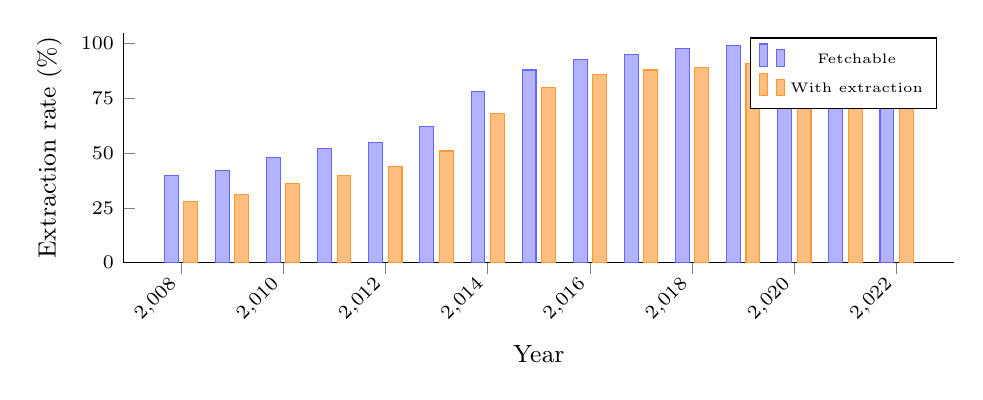
\begin{tikzpicture}
\begin{axis}[
    ybar,
    bar width=5pt,
    width=\columnwidth,
    height=4.5cm,
    xlabel={Year},
    ylabel={Extraction rate (\%)},
    ymin=0, ymax=105,
    xtick={2008,2010,2012,2014,2016,2018,2020,2022},
    xticklabel style={font=\scriptsize, rotate=45, anchor=east},
    ytick={0,25,50,75,100},
    yticklabel style={font=\scriptsize},
    xlabel style={font=\small},
    ylabel style={font=\small},
    legend style={font=\tiny, at={(0.98,0.98)}, anchor=north east},
    legend entries={Fetchable, With extraction},
    axis lines*=left,
    enlarge x limits=0.08,
]
% Fetchable rates (%) by year (approximate from era data)
\addplot[fill=blue!30, draw=blue!60] coordinates {
    (2008,40) (2009,42) (2010,48) (2011,52) (2012,55)
    (2013,62) (2014,78) (2015,88) (2016,93)
    (2017,95) (2018,98) (2019,99) (2020,99) (2021,99) (2022,100)
};
% With-extraction rates (%) by year
\addplot[fill=orange!50, draw=orange!80] coordinates {
    (2008,28) (2009,31) (2010,36) (2011,40) (2012,44)
    (2013,51) (2014,68) (2015,80) (2016,86)
    (2017,88) (2018,89) (2019,91) (2020,91) (2021,92) (2022,93)
};
\end{axis}
\end{tikzpicture}
\caption{Extraction rates by year across Project~KB (Study~2). Fetchability
(blue) rises sharply post-2013 as projects migrated to GitHub. Extraction
rate (orange) tracks closely once diffs are available, reaching 90\%+ for
2018--2022 entries.}
\label{fig:temporal}
\end{figure}

\textbf{Implication for future evaluations.}
The overall 76.4\% extraction rate across all 1{,}248 entries is a
conservative lower bound dominated by legacy infrastructure failures.
For the 916 entries published since 2014, the rate rises to 83.1\%;
for 2018--2022 entries alone it reaches 90.5\%.
Any future evaluation restricted to post-2017 advisories can therefore
expect extraction rates above 88\% without any improvements to the
extraction pipeline, simply due to improved repository accessibility.
This temporal boundary is a recommended filtering criterion for
practitioners building datasets from Project~KB.

\textbf{Interpretation.}
Because Project~KB does not always enumerate every affected construct
(some entries list only the fix commit with no construct-level annotation),
a strict function-name match between our output and KB's annotations
underestimates true recall.
Nevertheless, our 86.0\% extraction rate on fetchable diffs --- and 90.5\%
on the most recent advisory cohort --- demonstrates that automated patch
mining successfully identifies function-level content in the vast majority
of real-world security fix commits, across a corpus dramatically larger
than any prior automated evaluation.

% ══════════════════════════════════════════════════════════════
\section{Discussion}
\label{sec:discussion}

\subsection{Implications for Supply Chain Security}

Our results suggest that automated patch mining can upgrade SCA tools 
from package-level to function-level alerting for approximately two-thirds 
of advisories. The 84\% precision is sufficient for \emph{triage 
assistance}---prioritizing which CVE alerts to investigate first---though 
not yet for fully automated remediation decisions.

The 31\% of advisories that yield no functions reveal a systemic gap in 
vulnerability reporting: advisories that are fixed by dependency version 
bumps or configuration changes contain no code-level information by design. 
We argue that advisory databases should encourage reporters to provide 
function-level annotations when the fix involves source code changes.

\subsection{Limitations}

This work has several limitations that motivate future research:

\begin{itemize}
    \item \textbf{Recall upper bound unknown.} Project~KB does not
    enumerate all affected constructs for every entry; our 86.0\%
    extraction rate thus reflects coverage of fix-commit diffs, not
    a true recall against a complete function-level oracle.
    A future study with fully annotated ground truth would sharpen
    this estimate.
    \item \textbf{Regex-based extraction.} Our approach uses pattern
    matching rather than full AST parsing of diffs. This may miss
    complex constructs such as decorated functions, nested definitions,
    or macro-generated code.
    \item \textbf{Temporal bias.} Project~KB entries span 2005--2022,
    with 48\% of no-diff cases concentrated in 2008--2014 due to
    legacy Apache infrastructure. Modern repositories (2016--2022)
    have substantially higher fetchability.
    \item \textbf{Go and Rust not yet supported.} Extending to these
    ecosystems requires only new regex patterns and no architectural
    changes.
\end{itemize}

\subsection{Integration with Reachability Tools}

The mined function-level data integrates directly with tools that perform 
reachability analysis, such as Eclipse 
Steady~\cite{plate2015eclipsesteady} and the OSCAR 
platform~\cite{oscar-icsme}. When combined with static call graphs, 
patch mining enables a qualitatively different triage workflow: rather 
than ``Package X has a CVE,'' engineers receive ``Function Y in Package X 
has a CVE, and it is/is not reachable from your application's public API.''

% ══════════════════════════════════════════════════════════════
% ══════════════════════════════════════════════════════════════
\section{Dataset Release}
\label{sec:dataset}

To support reproducibility and future research, we release all artifacts
produced by this study as an open replication package.

\textbf{Contents.}
The package includes: (i)~the complete extraction output for all 1{,}248
Project~KB advisories (8{,}069 function names, per-entry confidence scores,
and failure-mode annotations); (ii)~the JS/Python extraction results for
45~GHSA advisories (133 functions); (iii)~the cross-ecosystem comparison
scripts and Project~KB cross-validation pipeline; and (iv)~the
language-specific regex modules for JS, Python, and Java.

\textbf{Formats.}
Extraction results are provided as \texttt{.csv} (one row per advisory,
with \texttt{vuln\_id}, \texttt{functions}, \texttt{confidence},
\texttt{failure\_mode}) and \texttt{.json} (structured with per-function
metadata including source file path and diff line number).
The dataset is schema-compatible with Project~KB's advisory format,
facilitating direct join operations for downstream studies.

\textbf{Availability.}
All data, scripts, and the patch mining pipeline are archived at:
\url{https://github.com/ANONYMIZED/oscar-research-data}
(DOI to be assigned upon acceptance via Zenodo).

% ══════════════════════════════════════════════════════════════
\section{Related Work}
\label{sec:related}

\textbf{Vulnerability Databases.}
The NVD~\cite{nvd} and OSV~\cite{osv} aggregate vulnerability data at the
package-version level.
GHSA provides additional metadata including fix commit links, which our
technique exploits.
None of these databases systematically provide function-level data.
Alfadel et al.~\cite{alfadel2022exploitability} studied the exploitability
of npm vulnerabilities and found that 59\% of advisories affect functions
that are reachable in at least one downstream consumer---reinforcing the
demand for function-level data that our pipeline supplies automatically.

\textbf{Manual Curation.}
Ponta et al.~\cite{ponta2019projectkb} introduced Project~KB, a manually
curated knowledge base mapping Java vulnerabilities to affected constructs.
While highly precise, manual curation does not scale to the tens of
thousands of advisories across multiple ecosystems.
Our automated approach complements Project~KB: we use it as ground truth
in Study~2, confirming 86.0\% extraction coverage on its 1{,}248 entries.

\textbf{Vulnerability Detection.}
Kim et al.~\cite{kim2017vuddy} proposed VUDDY, which detects cloned
vulnerable functions through code hashing.
Unlike VUDDY, our technique identifies the \emph{original} vulnerable
function from the fix commit rather than detecting clones in downstream
projects.
Dann et al.~\cite{dann2021identifying} systematically evaluated
open-source vulnerability scanners and found that most lack function-level
information entirely, confirming the gap our approach addresses.

\textbf{Commit Analysis.}
The SZZ algorithm~\cite{sliwerski2005szz} traces bug-introducing commits
from bug fixes.
Reis et al.~\cite{reis2021vszz} extended SZZ to security contexts
(V-SZZ), identifying vulnerability-introducing commits with higher
precision by filtering for security-relevant keywords.
Our work follows a similar intuition---exploiting fix commits as a source
of vulnerability information---but extracts \emph{function names} at the
patch site rather than tracing back to introducing commits.

\textbf{Reachability Analysis.}
Eclipse Steady~\cite{plate2015eclipsesteady} performs dynamic reachability
analysis for Java, consuming function-level vulnerability data as input.
Our technique automates the production of this input data across multiple
languages.
Pashchenko et al.~\cite{pashchenko2020qualitative} demonstrated that up to
73\% of SCA alerts may be for unreachable code, which underscores the
practical value of function-level data: once the vulnerable function is
known, reachability can be checked against static call graphs without
requiring the full application context.

% ══════════════════════════════════════════════════════════════
\section{Conclusion and Future Work}
\label{sec:conclusion}

We presented an automated, multi-language patch mining technique for
extracting function-level vulnerability data from security advisory fix
commits.
Across two evaluation studies, the technique achieved 69\% yield and
84\% precision on 45~npm and PyPI advisories, and an 86.0\% extraction
rate on 1{,}109~fetchable Java fix-commit diffs from the Project~KB
gold standard, recovering 8{,}069 unique function names.
These results demonstrate that automated patch mining is viable at
scale across multiple language ecosystems.

Future work includes: (1)~extending to Go and Rust with new regex
patterns; (2)~replacing regex-based extraction with full AST diff
analysis for improved handling of complex language constructs;
(3)~constructing a fully annotated function-level oracle beyond
Project~KB to enable true recall measurement; and
(4)~releasing a curated, DOI-assigned dataset of 8{,}000+
function-level CVE mappings as a community resource.

% ──────────────────────────────────────────────────────────────
\section*{Acknowledgments}

The development of the patch mining technique and this manuscript was
assisted by AI tools. All research methodology, pipeline design, and
interpretation of results are the intellectual contributions of the
human authors.

% ──────────────────────────────────────────────────────────────
\bibliographystyle{ACM-Reference-Format}
\begin{thebibliography}{12}

\bibitem{ohm2020backstabber}
M.~Ohm, H.~Plate, A.~Sykosch, and M.~Meier.
\newblock Backstabber's knife collection: A review of open source software 
supply chain attacks.
\newblock In \emph{Proc. DIMVA}, pages 23--43, 2020.

\bibitem{ladisa2023taxonomy}
P.~Ladisa, H.~Plate, M.~Martinez, and O.~Barais.
\newblock A taxonomy of attacks on open-source software supply chains.
\newblock In \emph{Proc. 44th IEEE S\&P}, pages 1509--1526, 2023.

\bibitem{pashchenko2020qualitative}
I.~Pashchenko, H.~Plate, S.~E.~Ponta, A.~Sabetta, and F.~Massacci.
\newblock Qualitative and quantitative analysis of the relationship between 
conditionally vulnerable cloned components.
\newblock \emph{IEEE Trans. Software Engineering}, 47(10):2136--2154, 2020.

\bibitem{ponta2019projectkb}
S.~E.~Ponta, H.~Plate, and A.~Sabetta.
\newblock A manually-curated dataset of fixes to vulnerabilities of 
open-source software.
\newblock In \emph{Proc. 16th MSR}, pages 383--387, 2019.

\bibitem{nvd}
NIST.
\newblock National Vulnerability Database, 2023.
\newblock \url{https://nvd.nist.gov}

\bibitem{osv}
Google.
\newblock OSV: Open Source Vulnerabilities, 2021.
\newblock \url{https://osv.dev}

\bibitem{plate2015eclipsesteady}
H.~Plate, S.~E.~Ponta, and A.~Sabetta.
\newblock Impact assessment for vulnerabilities in open-source software 
libraries.
\newblock In \emph{Proc. 31st ICSME}, pages 411--420, 2015.

\bibitem{kim2017vuddy}
S.~Kim, S.~Woo, H.~Lee, and H.~Oh.
\newblock VUDDY: A scalable approach for vulnerable code clone discovery.
\newblock In \emph{Proc. 38th IEEE S\&P}, pages 595--614, 2017.

\bibitem{sliwerski2005szz}
J.~{\'S}liwerski, T.~Zimmermann, and A.~Zeller.
\newblock When do changes induce fixes?
\newblock In \emph{Proc. 2nd MSR}, pages 1--5, 2005.

\bibitem{oscar-icsme}
Anonymous Authors.
\newblock Cross-level risk propagation in software supply chains:
A vision for bridging code and ecosystem analysis.
\newblock In \emph{Proc. 42nd ICSME (Visions)}, 2026.
\newblock \emph{Under review. Anonymized for double-blind review.}

\bibitem{zimmermann2019small}
M.~Zimmermann, C.-A.~Staicu, C.~Tenny, and M.~Pradel.
\newblock Small world with high risks: A study of security threats in the 
npm ecosystem.
\newblock In \emph{Proc. 28th USENIX Security}, pages 995--1010, 2019.

\bibitem{decan2019empirical}
A.~Decan, T.~Mens, and E.~Constantinou.
\newblock On the impact of security vulnerabilities in the npm package
dependency network.
\newblock In \emph{Proc. 15th MSR}, pages 181--191, 2018.

\bibitem{alfadel2022exploitability}
M.~Alfadel, D.~E.~Costa, and E.~Shihab.
\newblock Empirical analysis of the python package index (PyPI) ecosystem.
\newblock In \emph{Proc. 29th SANER}, pages 13--24, 2022.

\bibitem{dann2021identifying}
A.~Dann, B.~Hermann, and E.~Bodden.
\newblock Identifying challenges for OSS vulnerability scanners: A study and
tool suite.
\newblock In \emph{Proc. 36th IEEE/ACM ICSE}, 2021.

\bibitem{reis2021vszz}
S.~Reis, R.~Abreu, and L.~De-Almeida-Neto.
\newblock A ground-truth dataset and classification model for detecting
bug-introducing commits.
\newblock In \emph{Proc. 37th ICSME}, pages 1--12, 2021.

\end{thebibliography}

\end{document}
